\documentclass[a4paper,12pt]{article} % This defines the style of your paper

\usepackage[top = 2.5cm, bottom = 2.5cm, left = 2.5cm, right = 2.5cm]{geometry}

\usepackage[T1]{fontenc}
\usepackage[utf8]{inputenc}

\usepackage{multirow} % Multirow is for tables with multiple rows within one cell.
\usepackage{booktabs} % For even nicer tables.

\usepackage{mathtools}
\usepackage{graphicx}
\usepackage{tikz}
\usepackage{xcolor}

\usepackage{setspace}
\setlength{\parindent}{0in}

\usepackage{float}

\usepackage{fancyhdr}


\pagestyle{fancy} % With this command we can customize the header style.

\fancyhf{} % This makes sure we do not have other information in our header or footer.

\rhead{splay\_experiment \hfill Jiří Klepl}

\cfoot{\footnotesize \thepage}

\begin{document}

\thispagestyle{empty} % This command disables the header on the first page.

\begin{center}
	{\Large \bf Homework 6 - matrix\_experiment}
	\vspace{2mm}

	{\bf Jiří Klepl}

\end{center}

\vspace{0.4cm}


\setlength{\parindent}{2em}

\section{Prolog}

V následujících simulacích, čtyř simulovaných a jedné reálné, porovnáváme naivní implementaci (algoritmu ``řádek po řádku'') a cache-oblivious implementaci transponování čtvercové matice. Uvažovaná cache-oblivious implementace bude varianta algoritmu popisovaného na přednášce používající dvě subrutiny ($T$ a $TS$). Předpokládáme, že procházení podmatic je děláno v clockwise či anti-clockwise pořadí (a nikoliv v zašroubovávacím).

Sledovaným parametrem je průměrný počet cache-miss na přístup a jeho závislost na velikosti oné matice. Obě implementace provádějí shodné změny na zadané matici, ale v jiném pořadí. Při simulacích je uvažována jednovrstvá cache s LRU strategií.

\section{Simulované testy}

Jak bylo výše zmíněno, předpokládáme jednovrstvou cache s LRU strategií. Její velikost bude vždy udána parametrem $M$, velikost paměťových bloků (cache-line) potom parametrem $B$. Jeden experiment sestává z měření počtu cache-miss nad maticemi s rozměry $N \times N$, kde $N = 2^{\frac{i}{4}}; i \in \{20, 21, \dots 52\}$, vždy se stejnou cachí.

\subsection{Vedlejší efekty na výsledky}

Pro všechny simulace platí, že optimalizér kódu nehraje žádnou roli (nemusí totiž tomu tak být u reálných experimentů) a že testovaný kód dokonale popisuje uvažované výpočty.

Na druhou stranu, reálným vliv na výsledky má její příprava. Ta je prováděna metodou ``řádek po řádku'' a jejím efektem je uložení posledních několika bloků do simulované cache. U velkých matic (ve srovnání k velikosti cache) to nebude mít významný vliv, ale u malých matic to bude potenciálně znamenat snížený počet cache-miss a u analýzy výsledků by toto mělo být zohledněno. Zejména pokud se matice celé vejde do cache, nastanou falešně nulové výsledky.

Výše zmíněný efekt může být v reálných aplikacích využit pro optimalizace, ale stojí na domluvě mezi jednotlivými algoritmy (kde na dané matici začínají a končí) a tedy není předmětem naší analýzy.

Velmi podobný efekt vznikne, když je matice moc malá na to, aby strategie swappování měly dostatečný vliv na počet cache-miss, například, když se celá matice vejde do cache.

\subsection{Očekávané výsledky}
\label{expected}

\subsubsection{Odhad naivní implementace}

Pro všechny simulace bude očekávaný počet cache-miss na přístup u naivní implementace pracující nad dostatečně velkými maticemi přibližně roven $0.5$ (po krátkém vysvětlení uvedeme přesnější odhad). Toto pro nás bude sloužit jako horní limit, kterého lze jistě dosáhnout.

To plyne z toho, že při swapu je vždy jeden prvek pravděpodobně ve stejném bloku jako jeden z naposledy swappovaných prvků ($P_1 = \frac{1}{B}$), zatímco s ním swapovaný (s prohozenými souřadnicemi) je vždy v nenacachovaném bloku ($P_2 = 1$). Obojí dohromady má za výsledek průměrný počet cache-miss na přístup (bez ohledu na zarovnání):

\[P_{max} = \frac{B + 1}{2B} = 0.5 + \frac{1}{2B} \approx 0.5\]

\subsubsection{Dolní mez cache-miss}

Dolní hranice průměrného počtu cache-miss je rovna $\frac{1}{B}$. To jde ukázat tím, že je nutno načíst $\frac{N^2}{B}$ bloků paměti za $N^2$ přístupů, tedy minimální průměrný počet cache-miss na přístup je $P_{min} = \frac{\frac{N^2}{B}}{N^2} = \frac{1}{B}$. Dosažení tohoto limitu je možné, pokud jsou algoritmem práce na paměťových blocích dokonale spárovány (například, konkrétně v použitém algoritmu, se v nějaké hloubce matice rozdělí na zrcadlové dvojice podmatic (samozřejmě podle diagonály), kdy tyto dvojice dokonale pokryjí cache; lze jednoduše zobecnit).

\[P_{min} = \frac{1}{B}\]

\subsubsection{Horní odhad ideálního případu cache-oblivious implementace}

Horní odhad průměrného počtu cache-miss v ideálním případě je rovna $\frac{1}{B}$, je-li $2 B^2 \leq M$. Tedy, je-li cache po cache-line rozdělitelná na alespoň dva čtverce (tomu pak odpovídají zrcadlové dvojice podmatic, při počtu dělitelným čtyřmi virtuálně zdvojnásobíme cache-line), poté lze dosáhnout postupu popsaného výše. V opačném případě nalezneme mocninu dvou $B'$ takovou, že $2 B B' = M$, poté je horním odhadem ideálního případu $\frac{1}{B'} = \frac{2B}{M}$ a to odpovídá strategii, podobné minule diskutované, kdy však toto rozdělení tvoří použe podmnožina cache o velikosti $2 B'^2$, zbytek neužitečný, až na náhodné zlepšení.

\[P_{imax} = \begin{dcases}
	\frac{1}{B}, & \text{if } 2 B^2 \leq M\\
	\frac{2B}{M}, & \text{otherwise}
\end{dcases}
\]

\subsubsection{Horní mez neideálního případu cache-oblivious implementace}

Nejprve budeme uvažovat ``polo-ideální'' případ. U libovolné dvojice podmatic z ideálního případu, kdy matice měly rozměry shodné s paměťovými bloky, když myšleně posuneme bloky paměti přesně o polovinu a rozdělíme zmíněné podmatice, každou na čtyři další, každou teď prochází $\frac{2B'}{4} = \frac{B'}{2}$ unikátních paměťových bloků a danou dvojicí tedy vždy $B'$, tedy stejně, jako tomu bylo u původních podmatic v ideálním případě, tedy na celou dvojici podmatic je potřeba $4B'$ načtení namísto $2B'$. A toto lze dobře rozdělit LRU strategií cache.

Toto lze zobecnit pro libovolné posunutí bloků, kdy sousední dvojicí nových podmatic prochází maximálně $\frac{3B'}{2}$ paměťových bloků, tedy na celou původní podmatici $3B'$ načtení a na dvojici tedy $6B'$ načtení, to by nám dalo teoreticky trojnásobek ideálního odhadu, pokud stále zafunguje LRU strategie. Odpovědí je samozřejmě, že LRU strategie zafunguje, což lze snadno ukázat výčtem možností.

Fyzicky je samozřejmě daná dvojice původních podmatic stále na $4B'$ paměťových blocích. Tedy, vejdou-li se do cache, je horní mez dvojnásobkem meze ideálního případu.

Je-li $2 B' B = M$ a $B' < B$, pak bez újmy na obecnosti, za předpokladu, že všechny offsety řádků $\leq\frac{B'}{2}$, je každá druhá původní podmatice celá uvnitř $B'$ paměťových bloků, tedy máme čtyři možnosti, podle toho, jaké z původních podmatic z dané dvojice se vejdou celé do $B'$ bloků (lze si snadno ukázat, že na danou podmatici potřebujeme vždy $B'$ aktivně v cache), které jsou stejně pravděpodobné (u dostatečně velkých matic) a tedy dají nám horní mez $\frac{6B' + 2 \cdot 2 B' + 2 B'}{3 \cdot 2B'} = 2$, dvojnásobek meze ideálního případu.

Je-li $2 B^2 = M$, pak nelze bez znalosti konkrétního zarovnání a konfigurace cache vylepšit odhad trojnásobku a existují případy, kdy jej opravdu dosáhneme, není-li deterministicky dána priorita načtení matice (to ale v simulaci dáno je, tedy odhad bude vždy přesahovat).

Vše dohromady tedy:

\[
	P_{nmax} = \begin{dcases}
		2 P_{imax}, & \text{if } 4B^2 \leq M \vee \frac{M}{2B} < B\\
		3 P_{imax}, & \text{otherwise}
	\end{dcases}
\]

\subsection{Poznámka ke grafům}

Všechny grafy používají logaritmickou škálu o základu $2$ pro obě souřadnice. Souřadnice x je v logaritmické škále z důvodu zdůraznění periodicity vzhledem k logaritmu velikosti matice, souřadnice y z důvodu zvýraznění výsledků, neboť celá analýza hovoří o průměrném počtu cache-miss jako o násobcích určitých pravděpodobností a tedy je přirozenější používat škálu, kde násobky tvoří lineární zobrazení svých (taktéž logaritmicky zobrazených) složek.

\pagebreak

\subsection{Výsledky}
\label{results}

\begin{figure}[!htb]
	\caption{$M = 1024, B = 16$}
	\label{m1024b16}
	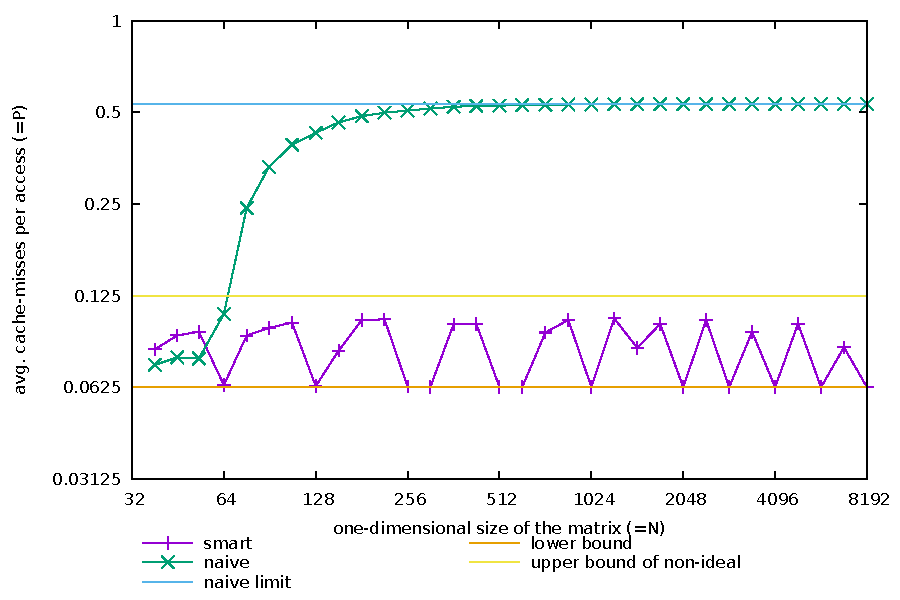
\includegraphics{sim-m1024-b16.pdf}
\end{figure}

Experiment zobrazen na figuře \ref{m1024b16} dobře reprezentuje případ, kdy $4B^2 \leq M$, tedy z pohledu ``chytré'' implementace (výše zmiňovaná cache-oblivious) se jedná o nejideálnější konfiguraci cache, kdy v zarovnaných (ideálních) případech dosahuje optimálního počtu cache-miss a v nezarovnaných je nejhůře dvakrát horší. Obě implementace se chovají podle očekávání.

Pro všechny limity a meze vizte část \ref{expected}.

\pagebreak

\begin{figure}[!hbt]
	\caption{$M = 8192, B = 64$}
	\label{m8192b64}
	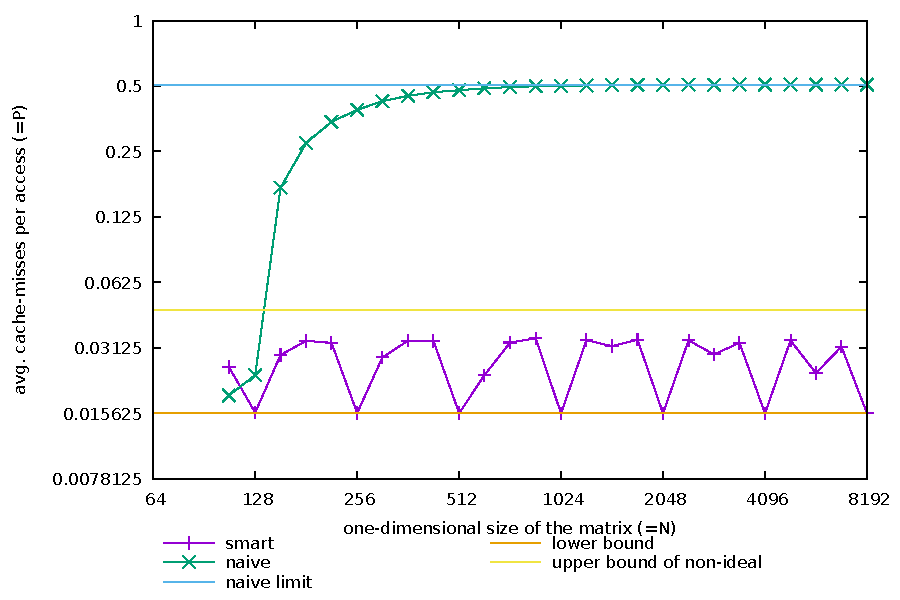
\includegraphics{sim-m8192-b64.pdf}
\end{figure}

Experiment zobrazen na figuře \ref{m8192b64} dobře zobrazuje případ, kdy je pro chytrou implementaci konfigurace cache ještě stále velice dobrá v ideálních případech a ve srovnání s nimi špatná v nezarovaných, neboť $2B^2 = M$ (vizte část \ref{expected}). Práce na nezarovnané matici může být doprovázen až trojnásobným počtem cache-miss.

Pro všechny limity a meze vizte část \ref{expected}.

\pagebreak

\begin{figure}[!hbt]
	\caption{$M = 65536, B = 256$}
	\label{m65536b256}
	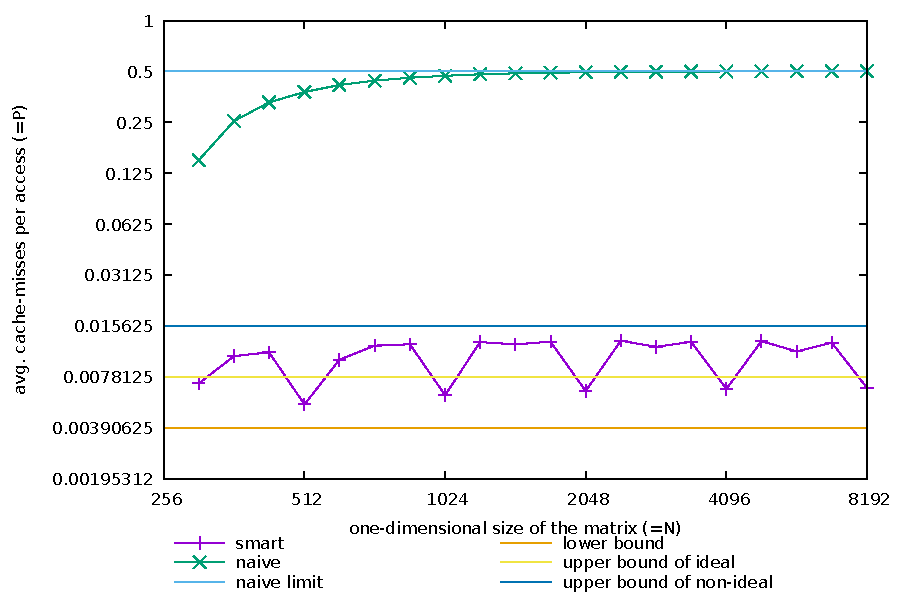
\includegraphics{sim-m65536-b256.pdf}
\end{figure}

Experiment zobrazen na figuře \ref{m65536b256} dobře zobrazuje případ, kdy je cache vzhledem k velikosti cache line moc malá ($M < 2B^2$), aby cache-oblivious algoritmus dosáhl optimálního počtu cache-miss, ale zato je nejhorší případ jen dvakrát horší, než je dvojnásobek nejlepšího.

Pro všechny limity a meze vizte část \ref{expected}.

\pagebreak

\begin{figure}[!hbt]
	\caption{$M = 65536, B = 4096$}
	\label{m65536b4096}
	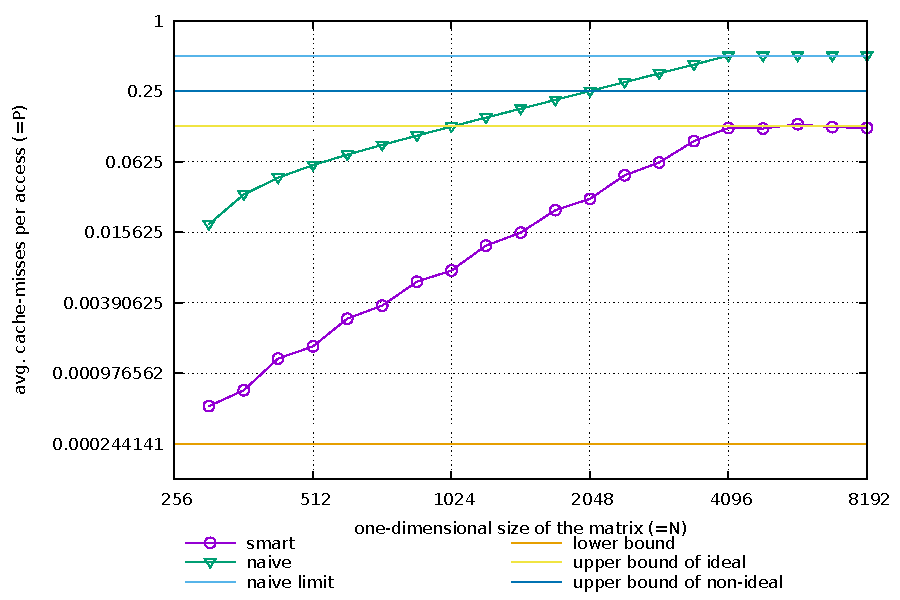
\includegraphics{sim-m65536-b4096.pdf}
\end{figure}

Experiment zobrazen na figuře \ref{m65536b4096} zobrazuje podobný případ, tomu minulému, ale je zde dobře pozorovatelný rozdíl mezi prací na malých a velkých maticích. Tento experiment uvažuje stejně velkou cache jako předešlý experiment zobrazený na figuře \ref{m65536b256}, ale zde algoritmus u dostatečně velkých matic dosahuje mnohem horších výsledků, neboť konfigurace zcela porušuje předpoklad návrhu algoritmu, že $M \geq 2 B^2$. U malých matic samozřejmě dosahuje velice dobrých výsledků (opět ve srovnání s předešlým experimentem), neboť jediným cache-miss je načtena významná část matice do cache.

Pro všechny limity a meze vizte část \ref{expected}.

\subsection{Zhodnocení}

V částech \ref{expected} a \ref{results} lze dobře vidět vliv zarovnanosti dat, velikosti paměťových bloků (cache-line) a konfigurace cache (pro tento algoritmus nejlépe $M \geq 2 B^2$).

Nejlepších výsledků bude dosaženo jedině na zarovnaných datech (či na extrémě malých maticích, kde strategie transponování není rozhodujícím faktorem) a výsledky jsou zlepšovány se zvětšováním velikosti cache-line (díky menšímu potřebnému počtu načtení) za udržení výše zmíněného předpokladu na konfiguraci cache.

\end{document}
